\documentclass[11pt,letterpaper]{article}
\usepackage[utf8]{inputenc}
\usepackage{amsmath,amssymb,fullpage,graphicx}

\let\hat\widehat
\let\tilde\widetilde
\begin{document}
\subsection*{Lect 3-1}
\subsection*{a}
\begin{verbatim}
set.seed(123)
nsample <- 100
x_obs <- rnorm(nsample,0,1)
y_obs <- rnorm(nsample,0,1)
delta_obs <- mean(x_obs) - mean(y_obs)
sigma_theo <- sqrt(1/nsample + 1/nsample)

>  1 - pnorm(delta_obs, 0, sigma_theo)
[1] 0.08079604
\end{verbatim}

The p-value is 0.08079604.

\subsection*{b}
\begin{verbatim}
pool <- c(x_obs, y_obs)
ntrial <- 1000
rand_delta <- numeric(ntrial)

for (i in 1:ntrial) {
 z = c(1:length(pool))
 samp_index <- sample(z, nsample, replace=F)
 samp_x <- pool[samp_index]
 samp_y <- pool[-samp_index]
 rand_delta[i] <- mean(samp_x) - mean(samp_y)
}
\end{verbatim}

The array named $" rand\_delta "$ is sample differences of means.

\subsection*{c}
\begin{verbatim}
hist(rand_delta, breaks = 20, xlab='Difference in Sample Means', 
    main = 'Randomization Sampling Distribution')
abline(v = delta_obs, col=2, lwd=2, lty=2)

rand_p <- length(rand_delta[rand_delta > delta_obs]) / ntrial
> rand_p
[1] 0.063
\end{verbatim}

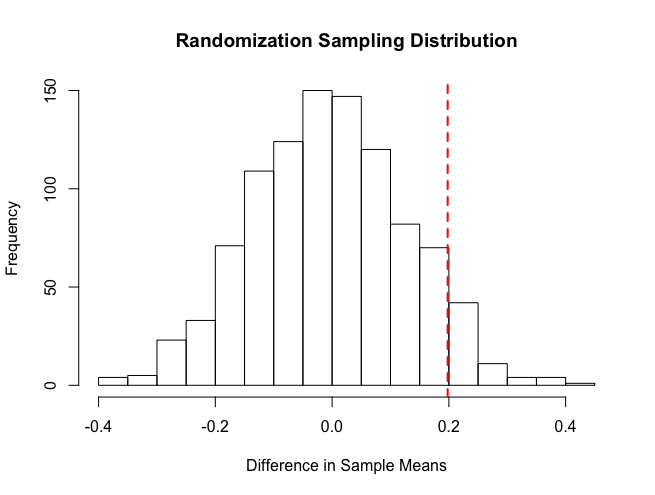
\includegraphics[scale=0.5]{lec-3-1-c.png}

The p-value of observed delta in sampling distribution is 0.063.

%\subsection*{Lect 3-2}
%\subsection*{a}
%\begin{align*}
%E_{X}[X] &= \int_{-\infty}^{\infty} \frac{t}{\sqrt{2 \pi \sigma^2}} \exp(-\frac{1}{2}(\frac{t - \mu}{\sigma})^2) dt \\
%&= \frac{1}{\sqrt{2 \pi}} \int_{-\infty}^{\infty} \frac{t}{\sigma} \exp(-\frac{1}{2} (\frac{t- \mu}{\sigma})^2) dt \\
%&= \frac{1}{\sqrt{2 \pi}} \int_{-\infty}^{\infty} (\frac{t - \mu}{\sigma} + \frac{\mu}{\sigma}) \exp(-\frac{1}{2} (\frac{t- \mu}{\sigma})^2) dt \\
%&= \frac{1}{\sqrt{2 \pi}} \int_{-\infty}^{\infty} (\frac{t - \mu}{\sigma} ) \exp(-\frac{1}{2} (\frac{t- \mu}{\sigma})^2) dt +  \frac{1}{\sqrt{2 \pi}} \int_{-\infty}^{\infty} (\frac{\mu}{\sigma} ) \exp(-\frac{1}{2} (\frac{t- \mu}{\sigma})^2) dt \\
%\text{Note that } 0 &= \frac{1}{\sqrt{2 \pi}} \int_{-\infty}^{\infty} (\frac{t - \mu}{\sigma} ) \exp(-\frac{1}{2} (\frac{t- \mu}{\sigma})^2) d(\frac{t - \mu}{\sigma}) \text{, for } (\frac{t - \mu}{\sigma}) \\
%\text{and } \frac{\sigma}{\sqrt{2 \pi}}  & \int_{-\infty}^{\infty} (\frac{t - \mu}{\sigma} ) \exp(-\frac{1}{2} (\frac{t- \mu}{\sigma})^2) d(\frac{t - \mu}{\sigma}) = \frac{1}{\sqrt{2 \pi}} \int_{-\infty}^{\infty} (\frac{t - \mu}{\sigma} ) \exp(-\frac{1}{2} (\frac{t- \mu}{\sigma})^2) dt \\
%\text{therefore } \sigma \cdot 0 &=  \frac{1}{\sqrt{2 \pi}} \int_{-\infty}^{\infty} (\frac{t - \mu}{\sigma} ) \exp(-\frac{1}{2} (\frac{t- \mu}{\sigma})^2) dt \\
%E_{X}[X] &= \frac{1}{\sqrt{2 \pi}} \int_{-\infty}^{\infty} (\frac{\mu}{\sigma} ) \exp(-\frac{1}{2} (\frac{t- \mu}{\sigma})^2) dt \\
%&= \frac{1}{\sqrt{2 \pi}} (\frac{\mu}{\sigma} ) \int_{-\infty}^{\infty} \exp(-\frac{1}{2} (\frac{t- \mu}{\sigma})^2) dt \\
%\text{Note that }  & \int_{-\infty}^{\infty} \exp(-\frac{1}{2} (\frac{t- \mu}{\sigma})^2) dt = \sigma \cdot \int_{-\infty}^{\infty} \exp(-\frac{1}{2} (\frac{t- \mu}{\sigma})^2) d(\frac{t - \mu}{\sigma}) \\
%E_{X}[X] &= \mu \cdot \frac{1}{\sqrt{2 \pi}} \int_{-\infty}^{\infty} \exp(-\frac{1}{2} (\frac{t- \mu}{\sigma})^2) d(\frac{t - \mu}{\sigma}) \\
%\text{Note that } 1 &=  \frac{1}{\sqrt{2 \pi}} \int_{-\infty}^{\infty} \exp(-\frac{1}{2} (\frac{t- \mu}{\sigma})^2) d(\frac{t - \mu}{\sigma}) \text{, for }( \frac{t - \mu}{\sigma}) \\
%\text{therefore, } & E_{X}[X] = \mu_{x}
%\end{align*}
%
%\subsection*{b}
%\begin{align*}
%E_{X}[X^2] &= \int_{-\infty}^{\infty} \frac{t^2}{\sqrt{2 \pi \sigma^2}} \exp(-\frac{1}{2}(\frac{t - \mu}{\sigma})^2) dt \\
%&= \int_{-\infty}^{\infty} \frac{(t^2 - 2 \mu t + \mu^2) + (2 \mu - \mu^2)}{\sqrt{2 \pi \sigma^2}} \exp(-\frac{1}{2}(\frac{t - \mu}{\sigma})^2) dt \\
%&= \int_{-\infty}^{\infty} \frac{(t^2 - 2 \mu t + \mu^2)}{\sqrt{2 \pi \sigma^2}} \exp(-\frac{1}{2}(\frac{t - \mu}{\sigma})^2) dt + \int_{-\infty}^{\infty} \frac{( 2 \mu t - \mu^2)}{\sqrt{2 \pi \sigma^2}} \exp(-\frac{1}{2}(\frac{t - \mu}{\sigma})^2) dt \\
%\end{align*}
%
%\begin{align*}
% \int_{-\infty}^{\infty} \frac{(t^2 - 2 \mu t + \mu^2)}{\sqrt{2 \pi \sigma^2}} \exp(-\frac{1}{2}(\frac{t - \mu}{\sigma})^2) dt &=  \int_{-\infty}^{\infty} \frac{(t - \mu)^2}{\sqrt{2 \pi \sigma^2}} \exp(-\frac{1}{2}(\frac{t - \mu}{\sigma})^2) dt \\
% &= \frac{\sigma^2}{\sqrt{2 \pi}}  \int_{\infty}^{-\infty} \frac{(t - \mu)^2}{\sigma^2} \exp(-\frac{1}{2}(\frac{t - \mu}{\sigma})^2) d(\frac{t - \mu}{\sigma}) \\
% &= \sigma^2 \cdot 1
%\end{align*}
%
%\begin{align*}
%\int_{-\infty}^{\infty} \frac{( 2 \mu t - \mu^2)}{\sqrt{2 \pi \sigma^2}} \exp(-\frac{1}{2}(\frac{t - \mu}{\sigma})^2) dt &= \int_{-\infty}^{\infty} \frac{( 2 \mu t)}{\sqrt{2 \pi \sigma^2}} \exp(-\frac{1}{2}(\frac{t - \mu}{\sigma})^2) dt - \int_{-\infty}^{\infty} \frac{( \mu^2)}{\sqrt{2 \pi \sigma^2}} \exp(-\frac{1}{2}(\frac{t - \mu}{\sigma})^2) dt \\
% &= 2 \mu \int_{-\infty}^{\infty} \frac{t}{\sqrt{2 \pi \sigma^2}} \exp(-\frac{1}{2}(\frac{t - \mu}{\sigma})^2) dt - \frac{\mu^2}{\sqrt{2 \pi \sigma^2}} \int_{-\infty}^{\infty} \exp(-\frac{1}{2}(\frac{t - \mu}{\sigma})^2) dt \\
%\text{from part a, we know } &  \int_{-\infty}^{\infty} \frac{t}{\sqrt{2 \pi \sigma^2}} \exp(-\frac{1}{2}(\frac{t - \mu}{\sigma})^2) dt = \mu \\
%\text{also note that } & \frac{1}{\sqrt{2 \pi}} \int_{-\infty}^{\infty} \exp(-\frac{1}{2}(\frac{t - \mu}{\sigma})^2) d(\frac{t - \mu}{\sigma}) = 1 \\
%\int_{-\infty}^{\infty} \frac{( 2 \mu t - \mu^2)}{\sqrt{2 \pi \sigma^2}} \exp(-\frac{1}{2}(\frac{t - \mu}{\sigma})^2) dt &= 2 \mu^2 - \mu^2
%\end{align*}
%
%\begin{align*}
%E_{X}[X] &= \sigma_{X}^2 + 2 \mu_{X}^2 - \mu_{X}^2 = \sigma_{x}^2 + \mu_{X}^2
%\end{align*}
%
%\subsection*{c}
%\begin{align*}
%E_{X^2}[X] &= \int_{-\infty}^{\infty} t \cdot f_{X^2}(t) dt \\
%&= \int_{-\infty}^{\infty} t \cdot 2^{-\frac{k}{2}} \frac{1}{\Gamma (\frac{k}{2})} t^{\frac{k}{2} - 1} \exp(-\frac{t}{2}) dt \\
%&= \int_{-\infty}^{\infty} 2^{-\frac{k}{2}} \frac{1}{\Gamma (\frac{k}{2})} t^{\frac{k}{2}} \exp(-\frac{t}{2}) dt \\
%&= 2^{-\frac{k}{2}} \frac{1}{\Gamma (\frac{k}{2})} \int_{-\infty}^{\infty} t^{\frac{k}{2}} \exp(-\frac{t}{2}) dt \\
%\end{align*}
%Integral by part, we get
%\begin{align*}
%\int_{-\infty}^{\infty} t^{\frac{k}{2}} \exp(-\frac{t}{2}) dt &= -2t^{\frac{k}{2}} \exp(-\frac{1}{2}t) |_{-\infty}^{\infty} + k \int_{-\infty}^{\infty} t^{\frac{k}{2} - 1} \exp(-\frac{t}{2}) dt \\
%\end{align*}
%Plug in the integral 
%\begin{align*}
%E_{X^2}[X] &= k \cdot 2^{-\frac{k}{2}} \frac{1}{\Gamma (\frac{k}{2})} \int_{-\infty}^{\infty} t^{\frac{k}{2} - 1} \exp(-\frac{t}{2}) dt \\
%&= k \cdot \int_{-\infty}^{\infty}2^{-\frac{k}{2}} \frac{1}{\Gamma (\frac{k}{2})}  t^{\frac{k}{2} - 1} \exp(-\frac{t}{2}) dt \\
%&= k \cdot \int_{-\infty}^{\infty} f_{X^2}(t) dt \\
%&= k 
%\end{align*}
%In this case $k$, the degree of freedom, is equal to 1, therefore, $E_{X^2}[X] = 1$
%
%\subsection*{d}
%\begin{align*}
%E_{X^2}[X^2] &= \int_{-\infty}^{\infty} t^2 \cdot f_{X^2}(t) dt \\
%&= \int_{-\infty}^{\infty} t^2 \cdot 2^{-\frac{k}{2}} \frac{1}{\Gamma (\frac{k}{2})} t^{\frac{k}{2} - 1} \exp(-\frac{t}{2}) dt \\
%&= \int_{-\infty}^{\infty} 2^{-\frac{k}{2}} \frac{1}{\Gamma (\frac{k}{2})} t^{\frac{k}{2} + 1} \exp(-\frac{t}{2}) dt \\
%&= 2^{-\frac{k}{2}} \frac{1}{\Gamma (\frac{k}{2})} \int_{-\infty}^{\infty} t^{\frac{k}{2} + 1} \exp(-\frac{t}{2}) dt \\
%\end{align*}
%Integral by part, we get
%\begin{align*}
%\int_{-\infty}^{\infty} t^{\frac{k}{2} + 1} \exp(-\frac{t}{2}) dt &= -2t^{\frac{k}{2} + 1} \exp(-\frac{1}{2}t) |_{-\infty}^{\infty} + (k + 2) \int_{-\infty}^{\infty} t^{\frac{k}{2}} \exp(-\frac{t}{2}) dt \\
%&= (k + 2) \int_{-\infty}^{\infty} t^{\frac{k}{2}} \exp(-\frac{t}{2}) dt
%\end{align*}
%\begin{align*}
%E_{X^2}[X^2] &= (k + 2) \cdot 2^{-\frac{k}{2}} \frac{1}{\Gamma (\frac{k}{2})} \int_{-\infty}^{\infty} t^{\frac{k}{2}} \exp(-\frac{t}{2}) dt \\
%&= (k + 2) \int_{-\infty}^{\infty} 2^{-\frac{k}{2}} \frac{1}{\Gamma (\frac{k}{2})} t^{\frac{k}{2}} \exp(-\frac{t}{2}) dt \\
%&= (k + 2) \cdot E_{X^2}(X) \\
%&= k^2 + 2k
%\end{align*}
%In this problem, degree of freedom is 1, therefore, $E_{X^2}[X^2] = 3$

\subsection*{Lect 3-2}
\begin{align*}
E_{Y}[y] &= \int_{-\infty}^{\infty} t \cdot f_Y (t) dt \\
&=  \int^{\infty}_{0} \frac{t}{2 \sqrt{t}}  ( f_X(\sqrt{t}) + f_X(- \sqrt{t}) ) dt + \int_{-\infty}^{0} 0 dt \\
&= \int^{\infty}_{0} \frac{t}{2 \sqrt{t}}   f_X(\sqrt{t}) dt + \int^{\infty}_{0} \frac{t}{2 \sqrt{t}}  f_X(-\sqrt{t}) dt
\end{align*}
Substitute $m, n$ for $\sqrt{t}, -\sqrt{t}$ in left-hand side of equation\\

\noindent The upper, lower bounds of integral turn to be $[0, \infty]$ for first half and $[-\infty,0]$ for the second half.
\begin{align*}
dm &= d(\sqrt{t}) = \frac{dt}{2 \sqrt{t}} = \frac{dt}{2m}\\
dn &= d(-\sqrt{t}) = -\frac{dt}{2 \sqrt{t}} = -\frac{dt}{2n}
\end{align*}
\begin{align*}
E_Y{Y} &= \int^{\infty}_{0} \frac{m^2}{2 m}   f_X(m) 2m \cdot dm + \int_{-\infty}^{0} - \frac{n^2}{2 n}  f_X(n) (-2n) \cdot dn \\
&= \int^{\infty}_{0} m^2 f_X(m) dm + \int_{-\infty}^{0} n^2 f_X(n) dn \\
&= \int^{\infty}_{-\infty} h^2 f_X(h) dh \text{ (h, m, n are all dummy variables of X)} \\
&= E_{X}[X^2]
\end{align*}


\subsection*{Lect 3-3}
Base on the definition of variance
\begin{align*}
V_{Y_1, Y_2}(Y_1 + Y_2) &= \int_{-\infty}^{\infty} \int_{-\infty}^{\infty} ( (t_1 + t_2) - E_{Y_1, Y_2}[t_1 + t_2] )^2 f_{Y_1,Y_2}(t_1, t_2) dt_1 dt_2 \\
\end{align*}
Based on the definition of expected value
\begin{align*}
E_{Y_1, Y_2}[Y_1 + Y_2] &= \int_{-\infty}^{\infty} \int_{-\infty}^{\infty} (t_1 + t_2) f_{Y_1, Y_2}(t_1, t_2) dt_1 dt_2 \\
&= \int_{-\infty}^{\infty} \int_{-\infty}^{\infty} t_1  f_{Y_1, Y_2}(t_1, t_2) dt_1 dt_2 + \int_{-\infty}^{\infty} \int_{-\infty}^{\infty} t_2  f_{Y_1, Y_2}(t_1, t_2) dt_1 dt_2 \\
&= \int_{-\infty}^{\infty} t_1 (\int_{-\infty}^{\infty} f_{Y_1, Y_2}(t_1, t_2) dt_2) dt_1 + \int_{-\infty}^{\infty} t_2 (\int_{-\infty}^{\infty} f_{Y_1, Y_2}(t_1, t_2) dt_1) dt_2
\end{align*}

Note that $\int_{-\infty}^{\infty} f_{Y_1, Y_2}(t_1, t_2) dt_2 = f_{Y_1}(Y_1)$ and $\int_{-\infty}^{\infty} f_{Y_1, Y_2}(t_1, t_2) dt_1 = f_{Y_2}(Y_2)$

\begin{align*}
E_{Y_1, Y_2}[Y_1 + Y_2] &= \int_{-\infty}^{\infty} t_1 f_{Y_1}(t_1) dt_1 +  \int_{-\infty}^{\infty} t_2 f_{Y_2}(t_2) dt_2 \\
&= E_{Y_1}(Y_1) + E_{Y_2}(Y_2)
\end{align*}

\begin{align*}
V_{Y_1, Y_2}(Y_1 + Y_2) &= \int_{-\infty}^{\infty} \int_{-\infty}^{\infty} ( t_1 + t_2 - E_{Y_1}(t_1) - E_{Y_2}(t_2))^2 f_{Y_1, Y_2}(t_1, t_2) dt_1 dt_2 \\
&= \int_{-\infty}^{\infty} \int_{-\infty}^{\infty} ( (t_1 - E_{Y_1}(t_1)) + (t_2 - E_{Y_2}(t_2))^2 f_{Y_1, Y_2}(t_1, t_2) dt_1 dt_2 \\
&= \int_{-\infty}^{\infty} \int_{-\infty}^{\infty} (t_1 - E_{Y_1}(t_1))^2 + (t_2 - E_{Y_2}(t_2))^2 + 2(t_1 + E_{Y_1}(t_1)(t_2 + E_{Y_1}(t_2))^2) f_{Y_1, Y_2}(t_1, t_2) dt_1 dt_2 \\
&= \int_{-\infty}^{\infty} \int_{-\infty}^{\infty} (t_1 - E_{Y_1}(t_1))^2 f_{Y_1, Y_2}(t_1, t_2) dt_1 dt_2 
+ \int_{-\infty}^{\infty} \int_{-\infty}^{\infty} (t_2 - E_{Y_2}(t_2))^2 f_{Y_1, Y_2}(t_1, t_2) dt_1 dt_2 \\
&+ \int_{-\infty}^{\infty} \int_{-\infty}^{\infty} 2(t_1 -  E_{Y_1}(t_1)(t_2 - E_{Y_1}(t_2)) f_{Y_1, Y_2}(t_1, t_2) dt_1 dt_2 \\
\end{align*}
Note that $\int_{-\infty}^{\infty} f_{Y_1, Y_2}(t_1, t_2) dt_2 = f_{Y_1}(Y_1)$ and $\int_{-\infty}^{\infty} f_{Y_1, Y_2}(t_1, t_2) dt_1 = f_{Y_2}(Y_2)$
\begin{align*}
\int_{-\infty}^{\infty} \int_{-\infty}^{\infty} (t_1 - E_{Y_1}(t_1))^2 f_{Y_1, Y_2}(t_1, t_2) dt_1 dt_2 &= \int_{-\infty}^{\infty}  (t_1 - E_{Y_1}(t_1))^2 f_{Y_1}(t_1) dt_1 \\
&= E_{Y_1}( Y_1 - E_{Y_1}(Y_1) ) \\
&= V_{Y_1}[Y_1]
\end{align*}
Similarly $\int_{-\infty}^{\infty} \int_{-\infty}^{\infty} (t_2 - E_{Y_2}(t_2))^2 f_{Y_1, Y_2}(t_1, t_2) dt_1 dt_2  = V_{Y_2}[Y_2]$ 
\begin{align*}
\int_{-\infty}^{\infty} \int_{-\infty}^{\infty} 2(t_1 -  E_{Y_1}(t_1)(t_2 - E_{Y_1}(t_2)) f_{Y_1, Y_2}(t_1, t_2) dt_1 dt_2 &= 2 \cdot E( E( Y_1 - E_{Y_1}(Y_1) ) ( Y_2 - E_{Y_2} )) \\
&= 2 \cdot Cov_{Y_1, Y_2} (Y_1, Y_2)
\end{align*}
Substitute $V_{Y_1}(Y_1)$, $V_{Y_2}(Y_2)$ and $Cov_{Y_1,Y_2} (Y_1, Y_2)$
\begin{align*}
V_{Y_1, Y_2}(Y_1 + Y_2) &= V_{Y_1}(Y_1) + V_{Y_1}(Y_2) + 2 \cdot Cov_{Y_1, Y_2}(Y_1, Y_2)
\end{align*}

\begin{align*}
V_{Y_1, Y_2}(Y_1 - Y_2) &= \int_{-\infty}^{\infty} \int_{-\infty}^{\infty} ( (t_1 - t_2) - E_{Y_1, Y_2}[t_1  - t_2] )^2 f_{Y_1,Y_2}(t_1, t_2) dt_1 dt_2 \\
&= \int_{-\infty}^{\infty} \int_{-\infty}^{\infty} ( (t_1 - E_{Y_1}(t_1)) - (t_2 - E_{Y_2}(t_2))^2 f_{Y_1, Y_2}(t_1, t_2) dt_1 dt_2 \\
&= \int_{-\infty}^{\infty} \int_{-\infty}^{\infty} (t_1 - E_{Y_1}(t_1))^2 f_{Y_1, Y_2}(t_1, t_2) dt_1 dt_2 
+ \int_{-\infty}^{\infty} \int_{-\infty}^{\infty} (t_2 - E_{Y_2}(t_2))^2 f_{Y_1, Y_2}(t_1, t_2) dt_1 dt_2 \\
&+ \int_{-\infty}^{\infty} \int_{-\infty}^{\infty} 2(t_1 -  E_{Y_1}(t_1)(t_2 - E_{Y_1}(t_2)) f_{Y_1, Y_2}(t_1, t_2) dt_1 dt_2 \\
&= V_{Y_1}(Y_1) + V_{Y_2}(Y_2) - 2 Cov_{Y_1, Y_2} (Y_1, Y_2)
\end{align*}

This proves $V_{Y_1, Y_2}(Y_1 \pm Y_2) = V_{Y_1}(Y_1) + V_{Y_2}(Y_2) \pm 2 Cov_{Y_1, Y_2}(Y_1, Y_2)$

%\begin{align*}
%V_{Y_1, Y_2}(Y_1 + Y_2) &= E_{Y_1, Y_2}[((Y_1 + Y_2) - E_{Y_1, Y_2}[Y_1 + Y_2])^2] \\
%&= E_{Y_1, Y_2}[ (Y_1 + Y_2 - E_{Y_1} - E_{Y_2})^2 ] \\
%&= E_{Y_1,Y_2} [ ((Y_1 - E_{Y_1}[Y_1]) + (Y_2 - E_{Y_2}[Y_2]))^2 ] \\
%&= E_{Y_1,Y_2} [ (Y_1 - E_{Y_1}[Y_1])^2 + 2 \cdot (Y_1 - E_{Y_1}[Y_1])(Y_2 - E_{Y_2}[Y_2]) + (Y_2 - E_{Y_2}[Y_2])^2] \\
%&= E_{Y_1} [(Y_1 - E_{Y_1}[Y_1])^2] + 2 \cdot E_{Y_1, Y_2} [ (Y_1 - E_{Y_1}[Y_1])(Y_2 - E_{Y_2}[Y_2]) ] + E_{Y_2} [ (Y_2 - E_{Y_2}[Y_2])^2  ]
%\end{align*}
%From the definition of variance and co-variance, we know that
%\begin{align*}
%Cov_{Y_1, Y_2} [Y_1, Y_2] &= E_{Y_1, Y_2} [ (Y_1 - E_{Y_1}[Y_1])(Y_2 - E_{Y_2}[Y_2]) ] \\
%V_{Y_1} [Y_1] &= E_{Y_1} [(Y_1 - E_{Y_1}[Y_1])^2] \\
%V_{Y_2} [Y_2] &= E_{Y_2} [(Y_2 - E_{Y_2}[Y_2])^2] 
%\end{align*}
%Plug in these substitutions, we get
%\begin{align*}
%V_{Y_1, Y_2}(Y_1 + Y_2) &= V_{Y_1} [Y_1] + 2\cdot Cov_{Y_1, Y_2}[Y_1, Y_2] + V_{Y_2}[Y_2]
%\end{align*}
%
%\begin{align*}
%V_{Y_1, Y_2}(Y_1 - Y_2) &= E_{Y_1, Y_2}[((Y_1 - Y_2) - E_{Y_1, Y_2}[Y_1 - Y_2])^2] \\
%&= E_{Y_1, Y_2}[ (Y_1 - Y_2 - E_{Y_1} + E_{Y_2})^2 ] \\
%&= E_{Y_1,Y_2} [ ((Y_1 - E_{Y_1}[Y_1]) - (Y_2 - E_{Y_2}[Y_2]))^2 ] \\
%&= E_{Y_1,Y_2} [ (Y_1 - E_{Y_1}[Y_1])^2 - 2 \cdot (Y_1 - E_{Y_1}[Y_1])(Y_2 - E_{Y_2}[Y_2]) + (Y_2 - E_{Y_2}[Y_2])^2] \\
%&= E_{Y_1} [(Y_1 - E_{Y_1}[Y_1])^2] - 2 \cdot E_{Y_1, Y_2} [ (Y_1 - E_{Y_1}[Y_1])(Y_2 - E_{Y_2}[Y_2]) ] + E_{Y_2} [ (Y_2 - E_{Y_2}[Y_2])^2  ] \\
%&= V_{Y_1}[Y_1] - 2 \cdot Cov_{Y_1, Y_2}[Y_1, Y_2] + V_{Y_2}[Y_2]
%\end{align*}
%
%This proves $V_{Y_1, Y_2}[Y_1 \pm Y_2] = V_{Y_1}[Y_1] + V_{Y_2}[Y_2] \pm 2Cov_{Y_1,Y_2}[Y_1, Y_2]$

\subsection*{Lect 4-1}
\begin{align*}
& \sum_i^n \frac{Y_i - \mu_Y}{\sigma_Y^2} \sim \chi_n^2   \text{, this step is correct} \\
& \sum_i^n \frac{\bar{Y} - \mu_Y}{\sigma_Y^2} \sim \chi_1^2  \text{, this step is correct as well} \\
& \text{Sign of }  \frac{2 (\bar{Y} - \mu_Y)}{\sigma^2} \sum_i^n (Y_i - \mu_Y)  \text{ should be negative } \\
& \text{The value of } \sum_i^n (Y_i - \mu_Y)  \text{ is not guaranteed equal to 0}
\end{align*}
\begin{align*}
- \frac{2 (\bar{Y} - \mu_Y)}{\sigma^2} \sum_i^n (Y_i - \mu_Y) &= - \frac{2 (\bar{Y} - \mu_Y)}{\sigma^2} (n \bar{Y} - n \mu_Y) \\
&= -2 \cdot (\frac{(\bar{Y} - \mu_Y)}{\sigma_Y / \sqrt{n}})^2 \\
&= -2 \cdot \chi^2_1
\end{align*}

\noindent Note that $2 \cdot \chi^2_1 \neq \chi^2_2$, and to prove $\sum_i^n \frac{Y_i - \mu_Y}{\sigma_Y^2} + \sum_i^n \frac{\bar{Y} - \mu_Y}{\sigma_Y^2} - \frac{2 (\bar{Y} - \mu_Y)}{\sigma^2} \sum_i^n (Y_i - \mu_Y) \sim \chi^2_{n-1}$ requires $\frac{2 (\bar{Y} - \mu_Y)}{\sigma^2} \sum_i^n (Y_i - \mu_Y)$ to follow $\chi^2_{2}$, therefore, this method does not work in proving $\frac{1}{\sigma^2_Y} \sum_i^n (Y_i - \bar{Y})^2 \sim \chi^2_{n-1}$ .

\subsection*{Lect 4-2}
We know the fact that $E_{Z}(Z_i)=0$ and $E_Z(Z_i^2) = 1$ \\

\noindent since Z is identically distributed, $E_Z(Z) = E_Z(Z_i) = 0$, $E_Z(Z^2) = E_Z(Z_i^2) = 1$\\

Let $ss$ denotes $\sum_i^n (Z_i - \bar{Z})^2$, then $E_Z(ss) = E_Z (\sum_i^n (Z_i - \bar{Z})^2)$

\begin{align*}
ss &= \sum_i^n z_i^2 - 2 \sum_i^n Z_i \cdot \bar{Z} + \sum_i^n \bar{Z} ^2 \\
&= n \cdot \bar{Z^2} - 2 n \bar{Z}^2 + n \bar{Z}^2 \\
&= n ( \bar{Z^2} - \bar{Z}^2 ) \\
E_Z(ss) &= n\cdot E_Z(\bar{Z^2} - \bar{Z}^2)
\end{align*}
\begin{align*}
E_Z(\bar{Z^2}) &= E_Z(\frac{1}{n} \sum_i^n Z_i^2) = \frac{1}{n} \sum_i^n E_Z(Z_i^2) \\
\text{Since Z is identical distributed, }  & E_Z(\bar{Z^2}) = \frac{1}{n} \sum_i^n E_Z(Z_i^2) = E_Z(Z^2) \frac{1}{n} \sum_i^n 1=  E_Z(Z^2) = 1
\end{align*}

\begin{align*}
E_Z(\bar{Z}^2) &= E_Z[ (\frac{1}{n} \sum_i^n Z_i) ( \frac{1}{n} \sum_j^n Z_j ) ] \\
&= \frac{1}{n^2} E_Z[(\sum_i^n Z_i)(\sum_j^n) Z_j)] \\
&= \frac{1}{n^2} E_Z( \sum_i^n Z_i^2 + 2 \cdot \sum_{i > j}^n Z_i Z_j) \\
&= \frac{1}{n^2} E_Z( \sum_i^n Z_i^2  ) + \frac{2}{n^2} E_Z(\sum_{i>j}^n Z_i Z_j) \\
&= \frac{1}{n^2}  \sum_i^nE_Z( Z_i^2  ) + \frac{2}{n^2}\sum_{i>j}^n E_Z( Z_i Z_j) 
\end{align*}
Since Z is independent, $ E_Z(Z_iZ_j) = E_Z(Z_i) E_Z(Z_j) $ \\

\noindent Since Z is identical distributed, $E_Z(Z_i) = E_Z(Z_j) = E_Z(Z) = 0$ \\

\noindent Therefore, $E_Z(Z_iZ_j) =  E_Z(Z_i) E_Z(Z_j) =0$, $E_Z(\bar{Z}^2) = \frac{1}{n^2} \cdot n + \frac{2}{n^2} \cdot n \cdot 0 = \frac{1}{n}$

\begin{align*}
E_Z(ss) &= n\cdot E_Z(\bar{Z^2} - \bar{Z}^2) \\
&= n\cdot E_Z(\bar{Z^2}) - nE_Z(\bar{Z}^2) \\
&= n \cdot 1 - n \cdot \frac{1}{n} \\
&= n - 1
\end{align*}

\subsection*{Lect 4-3}
\subsection*{a}
We have proved in class that $\frac{ss}{\sigma^2} \sim \chi^2_{n-1}$ and $\frac{ss}{n-1} = s^2$ \\

\noindent Therefore $\frac{(n - 1)s^2}{\sigma^2} \sim \chi^2_{n-1}$

\noindent P(sample variance $>$ 1.459) = P($\frac{(n-1)s^2}{\sigma^2} > \frac{(n-1) 1.459}{\sigma^2}$)

\begin{verbatim}
sigma2 <- 1
s2 <- 1.459
n = 31
test_stat <- (n-1)*s2 / sigma2
> 1 - pchisq(test_stat, df=n-1)
[1] 0.05003083
\end{verbatim}

\noindent P(sample variance $>$ 1.459) = 0.05003083

\subsection*{b}
From part a, we know that if we assume population variance is 1, the probability of observing sample variance greater than 1.459 is approximately 0.05. In other words, under $H_0$ of $\sigma^2 = 1$, p-value of 1.459 is 0.05.\\

\noindent Under null hypothesis of population variance equals 1, it is more extreme to observe sample variance of 1.6 than 1.459. Therefore, when observing sample variance of 1.6, it is implausible that population variance is 1 or less. 

\subsection*{Lect 5-1}
Let $s_1^2$ denotes sample variance of $Y$ under $X=1$.\\

\noindent Let $s_2^2$ denotes sample variance of $Y$ under $X=2$.\\

\noindent P($s_1^2 > 2.33 \cdot s_2^2$) = P($\frac{s_1^2}{s_2^2} > 2.33$) \\

\noindent Note that population variances of $Y$ under both $X=1,2$ are equivalent, therefore, $\frac{s_1^2}{s_2^2} \sim F_{df_1, df_2}$, where $df_1 = n_1-1 = 20$, $df_2 = n_2 - 1 = 24$.

\begin{verbatim}
n1 <- 21
n2 <- 25
> 1 - pf(2.33, df1=n1-1, df2=n2-1)
[1] 0.02484508
\end{verbatim}

\noindent P($s_1^2 > 2.33 \cdot s_2^2$) = 0.02484508

\subsection*{Lect 5-2}
\subsection*{a}
For $Y_{ij} = \mu + \epsilon_i + \epsilon_j$, $(Y_{1j} - Y_{2j}) = \mu + \epsilon_1 + \epsilon_j - (\mu + \epsilon_2 + \epsilon_j) = \epsilon_1 - \epsilon_2$ \\

\noindent For $Y_{ij} = \mu + \epsilon_i \epsilon_j$, $(Y_{1j} - Y_{2j}) = \mu + \epsilon_1 \epsilon_j - (\mu + \epsilon_2 \epsilon_j) = \epsilon_j (\epsilon_1 - \epsilon_2)$ \\

\noindent For $Y_{ij} = \mu_i + \epsilon_{ij}$, $(Y_{1j} - Y_{2j}) = \mu_1 + \epsilon_{1j} - (\mu_2 + \epsilon_{2j}) = (\mu_1 - \mu_2) + (\epsilon_{1j} - \epsilon_{2j})$ \\

\noindent For $Y_{ij} = \mu_{ij} + \epsilon_{ij}$, $(Y_{1j} - Y_{2j}) =  \mu_{1j} + \epsilon_{1j} - (\mu_{2j} + \epsilon_{2j}) = (\mu_{1j} - \mu_{2j}) + (\epsilon_{1j} - \epsilon_{2j})$ \\

\subsection*{b}
For $Y_{ij} = \mu + \epsilon_i + \epsilon_j$
\begin{align*}
E_Y(Y_{1j} - Y_{2j}) &= E_Y(\epsilon_1 - \epsilon_2) \\
&= E_Y(\epsilon_1) - E_Y(\epsilon_2)
\end{align*}
\noindent Note that $\epsilon$ is identical, $E(\epsilon_1) = E(\epsilon_2) = E(\epsilon) = 0$, then $E_Y(Y_{1j} - Y_{2j}) = 0$. \\

\noindent For $Y_{ij} = \mu + \epsilon_i \epsilon_j$
\begin{align*}
E_Y(Y_{ij} - Y_{2j}) &= E_Y( \epsilon_j (\epsilon_1 - \epsilon_2) ) \\
&= E_Y(\epsilon_1 \cdot \epsilon_j) - E_Y(\epsilon_2 \cdot \epsilon_j)
\end{align*}
\noindent Since $\epsilon_i$ is independently distributed, $E(\epsilon_1 \cdot \epsilon_j) = E(\epsilon_1) \cdot E(\epsilon_j)$ 
\begin{align*}
E_Y(Y_{ij} - Y_{2j}) &= E_Y(\epsilon_1) E_Y(\epsilon_j) - E_Y(\epsilon_j) E_Y(\epsilon_j) \\
&= 0 \\
\end{align*}

\noindent For $Y_{ij} = \mu_i + \epsilon_{ij}$
\begin{align*}
E_Y(Y_{1j} - Y_{2j}) &= E_Y((\mu_1 - \mu_2) + (\epsilon_{1j} - \epsilon_{2j})) \\
&= E_Y(\mu_1) - E_Y(\mu_2) + E_Y(\epsilon_{1j}) - E_Y(\epsilon_{2j}) \\
&= E_Y(\mu_1) - E_Y(\mu_2) \\
&= \mu_1 - \mu_2 \\
\end{align*}

\noindent For $Y_{ij} = \mu_{ij} + \epsilon_{ij}$
\begin{align*}
E_Y(Y_{1j} - Y_{2j}) &= E_Y((\mu_{1j} - \mu_{2j}) + (\epsilon_{1j} - \epsilon_{2j})) \\
&= E_Y(\mu_{1j}) -E_Y( \mu_{2j}) + E_Y(\epsilon_{1j}) - E_Y(\epsilon_{2j}) \\
&= E_Y(\mu_{1j}) -E_Y( \mu_{2j}) \\
&= \mu_{1j} - \mu_{2j} \\
\end{align*}

\subsection*{c}
The first two models, having $E(Y_{1j} - Y{2j})$ equal to zero, assume there are no difference between between two treatment means, i.e. $\mu_1 = \mu_2$. \\

\noindent The third model, with $E(Y_{1j} - Y{2j}) = \mu_1 - \mu_2$, considers the effect from treatment factor have on mean values. $\mu_1$ and $\mu_2$ represent population means when treatment factor is on level 1 and level 2. If difference do exist between these two population means, the difference can be shown by the model. \\

\noindent The forth model, with $E_Y(Y_{1j} - Y_{2j}) = \mu_{1j} - \mu_{2j}$, considers both effect from treatment factor and replication on mean value. The model assumes difference in mean exist both between levels of treatment factor and between times of replication. 

\subsection*{Lect 5-3}

We may set : \\
$H_0$: the tires are unsafe, i.e. true mean of pressure is greater than 10, $\mu > 10$ \\
$H_1$: the tires are safe, i.e. true mean of pressure is less than 10, $\mu \leq 10$\\

\noindent To reject in favor of the alternative, we are seeking evidence that sample mean pressure has a small p-value under the assumption that null is true. \\

\noindent In this case, it is intuitively worse to say the tires are safe but they are truly unsafe, therefore, the bad error is the evidence that the tires are safe, but in fact they are unsafe. Type two error is the failure to find evidence that tires are safe but they are truly safe. \\

\subsection*{Lect 5-4}
$(1-\alpha)$ CI for q$th$ quantile of $N(\mu, \sigma^2)$ can be represented as probability equation.

\begin{align*}
& P(T_{\frac{\alpha}{2}, n-1, \Delta} < T < T_{1-\frac{\alpha}{2}, n-1, \Delta}) = 1- \alpha \\
& P(T_{\frac{\alpha}{2}, n-1, \Delta} < \frac{\frac{\bar{Y} - \mu }{\sigma / \sqrt{n}} + \Delta}{\sqrt{X / n-1}} < T_{1-\frac{\alpha}{2}, n-1, \Delta}) = 1- \alpha \\
\end{align*}

\noindent Substitute $X = \frac{(n-1) s^2}{\sigma^2}$ for for $X$

\begin{align*}
& P(T_{\frac{\alpha}{2}, n-1, \Delta} < \frac{\frac{\bar{Y} - \mu }{\sigma / \sqrt{n}} + \Delta}{\sqrt{\frac{(n-1) s^2}{\sigma^2} / n-1}} < T_{1-\frac{\alpha}{2}, n-1, \Delta}) = 1- \alpha \\
& P(T_{\frac{\alpha}{2}, n-1, \Delta} < \frac{\frac{\bar{Y} - \mu }{\sigma / \sqrt{n}} + \Delta}{\sqrt{\frac{s^2}{\sigma^2}}} < T_{1-\frac{\alpha}{2}, n-1, \Delta}) = 1- \alpha \\
& P(T_{\frac{\alpha}{2}, n-1, \Delta} < \frac{\frac{\bar{Y} - \mu }{\sigma / \sqrt{n}} + \Delta}{\frac{s}{\sigma}} < T_{1-\frac{\alpha}{2}, n-1, \Delta}) = 1- \alpha \\
& P(T_{\frac{\alpha}{2}, n-1, \Delta} < \frac{\frac{\bar{Y} - \mu }{1 / \sqrt{n}} + \sigma  \Delta}{s} < T_{1-\frac{\alpha}{2}, n-1, \Delta}) = 1- \alpha \\
& P(s \cdot T_{\frac{\alpha}{2}, n-1, \Delta} < \frac{\bar{Y} - \mu }{1 / \sqrt{n}} + \sigma  \Delta < s \cdot T_{1-\frac{\alpha}{2}, n-1, \Delta}) = 1- \alpha \\
& P(s \cdot T_{\frac{\alpha}{2}, n-1, \Delta} < (\bar{Y} - \mu) \sqrt{n}  + \sigma  \Delta < s \cdot T_{1-\frac{\alpha}{2}, n-1, \Delta}) = 1- \alpha \\
& P(\frac{s}{\sqrt{n}} \cdot T_{\frac{\alpha}{2}, n-1, \Delta} < \bar{Y} - \mu + \frac{\sigma  \Delta}{\sqrt{n}}  < \frac{s}{\sqrt{n}} \cdot T_{1-\frac{\alpha}{2}, n-1, \Delta}) = 1- \alpha \\
& P(\frac{s}{\sqrt{n}} \cdot T_{\frac{\alpha}{2}, n-1, \Delta} - \bar{Y} < - \mu + \frac{\sigma  \Delta}{\sqrt{n}}  < \frac{s}{\sqrt{n}} \cdot T_{1-\frac{\alpha}{2}, n-1, \Delta} - \bar{Y}) = 1- \alpha \\
& P(\bar{Y} - \frac{s}{\sqrt{n}} \cdot T_{1-\frac{\alpha}{2}, n-1, \Delta} < \mu - \frac{\sigma \Delta}{\sqrt{n}} <  \bar{Y} - \frac{s}{\sqrt{n}} \cdot T_{\frac{\alpha}{2}, n-1, \Delta} ) = 1 - \alpha 
\end{align*}
\noindent Let $- \frac{\sigma \Delta}{\sqrt{n}} = \sigma Z_q$, which is substituting $- Z_q \sqrt{n}$ for $\Delta$ where $Z_q$ is a number depends only on $q$
\begin{align*}
& P(\bar{Y} - \frac{s}{\sqrt{n}} \cdot T_{1-\frac{\alpha}{2}, n-1, - Z_q \sqrt{n}} < \mu + \sigma Z_q <  \bar{Y} - \frac{s}{\sqrt{n}} \cdot T_{\frac{\alpha}{2}, n-1, - Z_q \sqrt{n}} ) = 1 - \alpha 
\end{align*}
\noindent The $(1 - \alpha)$ Confidence Interval for q$th$ quantile of $N(\mu, \sigma^2)$ is \\

$[\bar{Y} - \frac{s}{\sqrt{n}} \cdot T_{1-\frac{\alpha}{2}, n-1, - Z_q \sqrt{n}},  \bar{Y} - \frac{s}{\sqrt{n}} \cdot T_{\frac{\alpha}{2}, n-1, - Z_q \sqrt{n}}]$ 



\end{document}